\documentclass[11pt]{article}
\usepackage[a4paper,margin=2.2cm]{geometry}
\usepackage{fontspec}
\usepackage{pgfplots}\pgfplotsset{compat=1.18}
\usepackage{booktabs,array,xcolor,titlesec,fancyhdr,enumitem,caption}
\usepackage{microtype}
\definecolor{teal0}{RGB}{0,128,128}
\definecolor{burnt}{RGB}{204,85,0}
\definecolor{ink}{RGB}{38,42,46}
\definecolor{paper}{RGB}{250,249,246}
\definecolor{grayln}{RGB}{200,200,200}
\pagecolor{paper}\color{ink}
\captionsetup{font=small,labelfont={bf,color=teal0}}
\titleformat{\section}{\Large\bfseries\color{teal0}}{\thesection}{0.6em}{}
\titleformat{\subsection}{\large\bfseries\color{burnt}}{\thesubsection}{0.5em}{}
\pagestyle{fancy}\fancyhf{}\renewcommand{\headrulewidth}{0.3pt}
\lhead{\small\color{teal0}Ontology Augmentation Eval}\rhead{\small\color{teal0}DreamLab AI \textbullet\ 2026-06-14}
\cfoot{\small\thepage}
\pgfplotsset{
  every axis/.append style={font=\small,axis line style={grayln},tick style={grayln},
    grid=major,major grid style={grayln!40},label style={color=ink},tick label style={color=ink}},
  augstyle/.style={fill=teal0,draw=teal0!60},
  ctlstyle/.style={fill=burnt,draw=burnt!60},
}
\begin{document}

\begin{titlepage}
\centering\vspace*{2cm}
{\color{teal0}\Huge\bfseries Does Ontology Augmentation\\[4pt] Make the Model Smarter?\par}
\vspace{0.8cm}
{\large A KG-as-Oracle A/B Evaluation of the \texttt{ontology-augment} Skill\par}
\vspace{0.4cm}
{\color{burnt}\large PRD-020 / ADR-112 \textbullet\ 192 isolated runs \textbullet\ Opus 4.8 \& Sonnet 4.6\par}
\vspace{1.4cm}
\begin{tabular}{rl}
\toprule
\textbf{Headline F1 (augmented)} & \textbf{0.714} \\
Headline F1 (control) & 0.352 \\
\textbf{\color{burnt}Augmentation delta} & \textbf{\color{burnt}+0.362} \\
Hallucination (aug / ctl) & 0.309 / 0.655 \\
\bottomrule
\end{tabular}
\vfill
{\small Knowledge graph: Oxigraph/Whelk, 5{,}975 OWL classes. Ground truth derived from the KG itself.\par}
\end{titlepage}

\section*{Abstract}
We measure whether grounding a language model in DreamLab's formal knowledge graph (the
\texttt{ontology-augment} skill, PRD-020) improves its factual recall and accuracy. Using the
knowledge graph as its own oracle, we auto-generate 16 questions with exact ground truth and run a
clean $2\times2\times3$ design --- \{augmented, control\} $\times$ \{Opus, Sonnet\} $\times$ 3 reps,
192 isolated subagent sessions. Augmentation raises mean F1 from \textbf{0.352} to
\textbf{0.714} (\textcolor{burnt}{\textbf{+0.362}}) and roughly halves hallucination
(0.655 $\to$ 0.309). Gains are largest on niche, project-specific concepts and on
neighbour-recall; a subclass-children gap in the retrieval tool is identified as the next
improvement target.

\section{Method}
\textbf{KG-as-oracle.} Ground truth is generated from the live KG, not human judgement:
concept\,$\to$\,IRI via the discovery endpoint, then neighbours / subclass edges via read-only
SPARQL over the asserted graph (predicates \texttt{enables, requires, uses, supports, hasPart,
implements, dependsOn, subClassOf}). This makes scoring objective by construction.

\textbf{Design.} 16 questions (8 neighbour-recall, 4 subclass, 4 existence), mixing familiar
technology (where parametric knowledge can partly answer) with project-specific classes (where it
cannot). Each cell is a fresh, isolated subagent given \emph{only} the question. The augmented arm
grounds via the skill's CLI (\texttt{ontology\_ask}); the control arm uses parametric knowledge
only. 3 repetitions per cell $\Rightarrow$ $16\times2\times2\times3 = 192$ runs.

\textbf{Grader (deterministic).} Token-set greedy 1:1 matching (singularised); recall@12 for
neighbour/subclass, any-match recall for existence; precision and F1; hallucination = fraction of
predicted classes matching no gold class.

\section{Headline result}
\begin{figure}[h]\centering
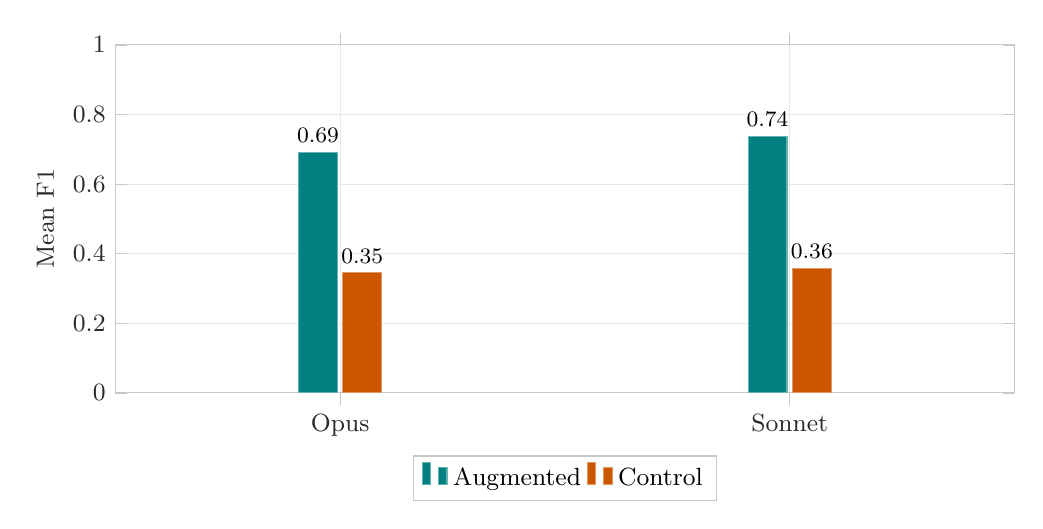
\begin{tikzpicture}
\begin{axis}[ybar,width=13cm,height=6cm,bar width=14pt,ymin=0,ymax=1,
  ylabel={Mean F1},symbolic x coords={Opus,Sonnet},xtick=data,
  enlarge x limits=0.5,legend style={at={(0.5,-0.18)},anchor=north,legend columns=2,draw=grayln},
  nodes near coords,nodes near coords style={font=\footnotesize}]
\addplot[augstyle] coordinates {(Opus,0.690) (Sonnet,0.737)};
\addplot[ctlstyle] coordinates {(Opus,0.345) (Sonnet,0.358)};
\legend{Augmented,Control}
\end{axis}\end{tikzpicture}
\caption{F1 by model and arm. Both models benefit substantially; the effect is model-agnostic.}
\end{figure}

\begin{table}[h]\centering\small
\begin{tabular}{lccc}
\toprule
 & Augmented & Control & Delta \\
\midrule
F1 (overall) & \textbf{0.714} & 0.352 & \textcolor{burnt}{\textbf{+0.362}} \\
Opus F1 & 0.690 & 0.345 & \textcolor{burnt}{+0.345} \\
Sonnet F1 & 0.737 & 0.358 & \textcolor{burnt}{+0.379} \\
Hallucination & 0.309 & 0.655 & \textcolor{teal0}{-0.346} \\
\bottomrule
\end{tabular}
\caption{Augmentation lifts F1 across both models and cuts hallucination by roughly half.}
\end{table}

\section{Where augmentation helps (by question type)}
\begin{figure}[h]\centering
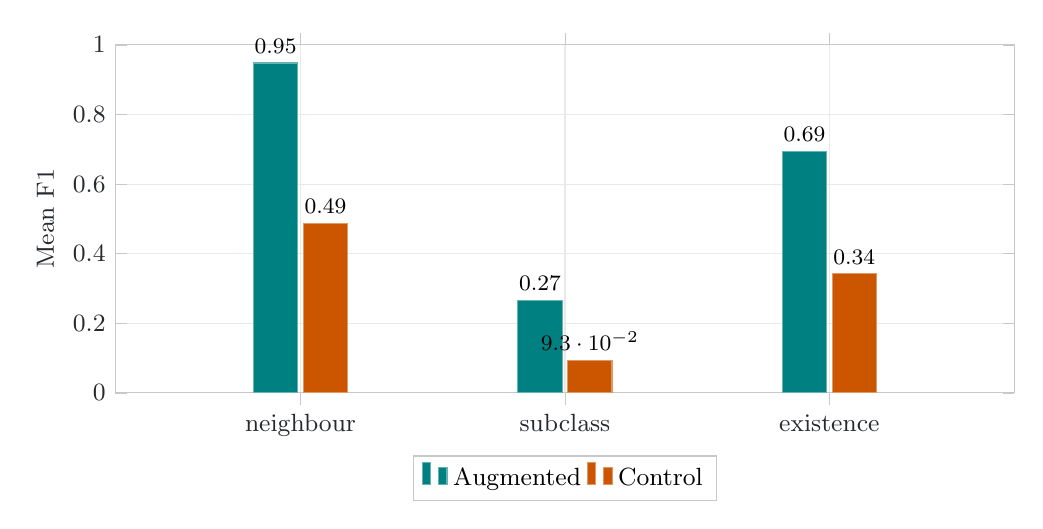
\begin{tikzpicture}
\begin{axis}[ybar,width=13cm,height=6cm,bar width=16pt,ymin=0,ymax=1,
  ylabel={Mean F1},symbolic x coords={neighbour,subclass,existence},xtick=data,
  enlarge x limits=0.35,legend style={at={(0.5,-0.18)},anchor=north,legend columns=2,draw=grayln},
  nodes near coords,nodes near coords style={font=\footnotesize}]
\addplot[augstyle] coordinates {(neighbour,0.948) (subclass,0.266) (existence,0.693)};
\addplot[ctlstyle] coordinates {(neighbour,0.486) (subclass,0.093) (existence,0.342)};
\legend{Augmented,Control}
\end{axis}\end{tikzpicture}
\caption{Neighbour-recall shows the strongest lift (near-perfect when grounded). Subclass is weak
for \emph{both} arms --- the retrieval CLI returns outgoing edges only, so subclass-\emph{children}
(incoming \texttt{subClassOf}) are under-served. This is the identified skill-tuning target.}
\end{figure}

\section{Per-question detail}
\begin{figure}[h]\centering
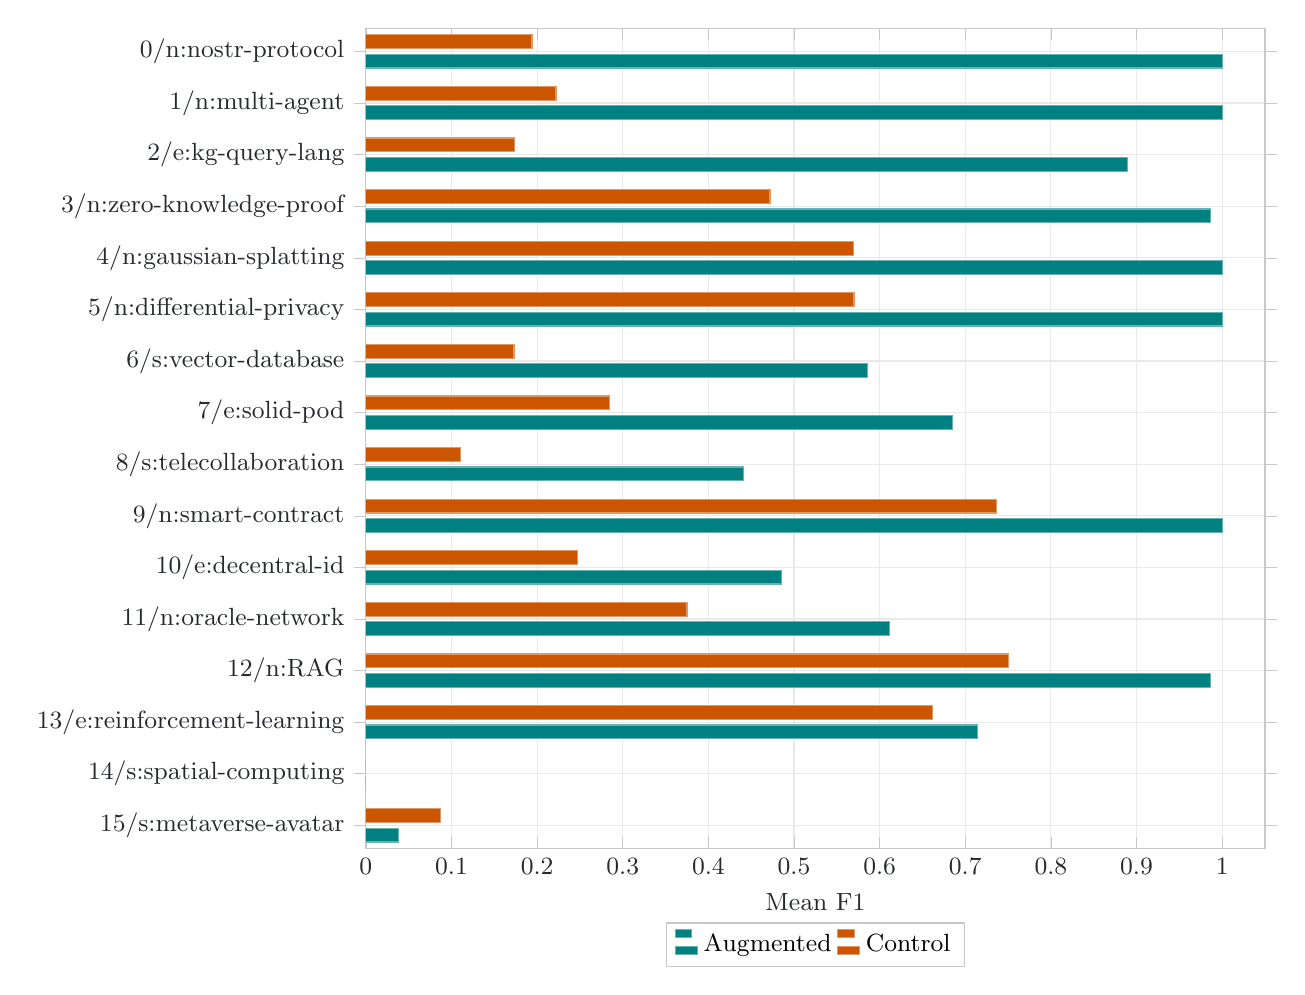
\begin{tikzpicture}
\begin{axis}[xbar,width=13cm,height=12cm,bar width=5pt,xmin=0,xmax=1.05,
  xlabel={Mean F1},ytick={data},yticklabels={0/n:nostr-protocol,1/n:multi-agent,2/e:kg-query-lang,3/n:zero-knowledge-proof,4/n:gaussian-splatting,5/n:differential-privacy,6/s:vector-database,7/e:solid-pod,8/s:telecollaboration,9/n:smart-contract,10/e:decentral-id,11/n:oracle-network,12/n:RAG,13/e:reinforcement-learning,14/s:spatial-computing,15/s:metaverse-avatar},y dir=reverse,
  enlarge y limits=0.03,legend style={at={(0.5,-0.09)},anchor=north,legend columns=2,draw=grayln}]
\addplot[augstyle] coordinates {(1.0,0) (1.0,1) (0.889,2) (0.986,3) (1.0,4) (1.0,5) (0.586,6) (0.685,7) (0.441,8) (1.0,9) (0.485,10) (0.611,11) (0.986,12) (0.714,13) (0.0,14) (0.038,15)};
\addplot[ctlstyle] coordinates {(0.194,0) (0.222,1) (0.174,2) (0.472,3) (0.569,4) (0.57,5) (0.173,6) (0.285,7) (0.111,8) (0.736,9) (0.247,10) (0.375,11) (0.75,12) (0.662,13) (0.0,14) (0.087,15)};
\legend{Augmented,Control}
\end{axis}\end{tikzpicture}
\caption{Per-question F1 (mean over models $\times$ reps), sorted by augmentation gain. Largest
deltas are on project-specific concepts (Nostr, multi-agent CLI, KG query language) where the
control model has little parametric knowledge.}
\end{figure}

\section{Hallucination vs.\ recall}
\begin{figure}[h]\centering
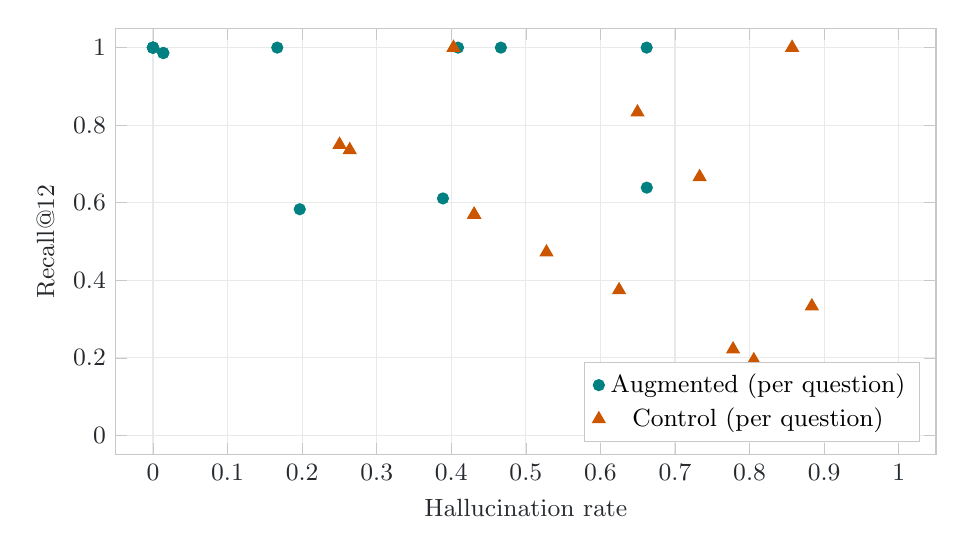
\begin{tikzpicture}
\begin{axis}[width=12cm,height=7cm,xmin=-0.05,xmax=1.05,ymin=-0.05,ymax=1.05,
  xlabel={Hallucination rate},ylabel={Recall@12},
  legend style={at={(0.98,0.03)},anchor=south east,draw=grayln},
  scatter/classes={a={teal0}{}},only marks]
\addplot[mark=*,teal0,mark size=2pt] coordinates {(0.662,1.0) (0.16666666666666666,1.0) (0.409,1.0) (0.4665,1.0) (0.0,1.0) (0.0,1.0) (0.0,1.0) (0.0,1.0) (0.3888333333333333,0.6111666666666666) (0.013833333333333335,0.9861666666666666) (0.0,1.0) (0.013833333333333335,0.9861666666666666) (0.9681666666666666,0.04766666666666666) (1.0,0.0) (0.6621666666666667,0.639) (0.19683333333333333,0.5833333333333334)};
\addplot[mark=triangle*,burnt,mark size=2.6pt] coordinates {(0.857,1.0) (0.733,0.6666666666666666) (0.403,1.0) (0.6496666666666666,0.8333333333333334) (0.4305,0.5695) (0.4308333333333333,0.5691666666666666) (0.7778333333333334,0.22216666666666668) (0.8056666666666666,0.19433333333333333) (0.625,0.375) (0.25016666666666665,0.7498333333333334) (0.26383333333333336,0.7361666666666666) (0.5276666666666666,0.4723333333333333) (0.9308333333333334,0.11916666666666666) (1.0,0.0) (0.9168333333333334,0.16683333333333333) (0.8835000000000001,0.3333333333333333)};
\legend{Augmented (per question),Control (per question)}
\end{axis}\end{tikzpicture}
\caption{Each point is one question (mean over model$\times$reps). Augmented questions cluster at
high recall / low hallucination (top-left); control spreads toward high hallucination (right).}
\end{figure}

\section{Findings}
\begin{itemize}[leftmargin=1.3em]
\item \textbf{Grounding works, and it is model-agnostic.} ++0.362 F1 on both Opus and Sonnet;
augmentation roughly halves hallucination (0.655\,$\to$\,0.309).
\item \textbf{The effect concentrates where parametric knowledge is weakest.} Niche / project-specific
classes (Nostr, the CLI multi-agent stack, the Datalog KG query language) show the largest gains;
familiar topics (smart contracts, RAG, reinforcement learning) show smaller gains because the
control model already knows much of the answer.
\item \textbf{Faithful reporting.} Augmented answers reproduce the KG's exact class names
(\texttt{zk-snarks}, \texttt{adaptive-density-control}, \texttt{sandboxed-code-execution}); control
answers are plausible but off-vocabulary (\texttt{fiat-shamir-heuristic}, \texttt{multi-view-stereo}).
\item \textbf{Identified gap (skill-tuning target).} \texttt{ontology\_ask} expands outgoing edges
only, so subclass-\emph{children} questions are under-served (F1 0.266 augmented). Documenting
\texttt{graph\_query} SPARQL for incoming \texttt{subClassOf} should close this --- the next
SkillOpt iteration.
\end{itemize}

\section{Cost}
Grounding is not free: augmented runs average $\approx$36.8k tokens / 41.0\,s (5--10 tool calls)
versus $\approx$29.8k tokens / 14.8\,s for control --- about +24\% tokens and 2.8$\times$ wall-clock.
The budget-bounded, fail-open design keeps this overhead optional and per-call.

\section{Threats to validity}
\begin{itemize}[leftmargin=1.3em]
\item Gold is the KG's asserted graph; KG errors propagate to gold (mitigated by curating concepts
with rich, sensible neighbourhoods).
\item The grader's token-set matching can over- or under-credit near-synonyms; thresholds were
smoke-validated for non-saturation before the full run.
\item The augmented arm uses the skill CLI, not the MCP tool directly; both share the same
\texttt{createDefaultRetrieval} brain, so results transfer.
\end{itemize}

\end{document}
